\documentclass[11pt,a4paper]{article}
\usepackage[utf8]{vietnam}
\usepackage{amsmath,amssymb}
\usepackage{tabularx}
\usepackage{tikz}
\usepackage{xcolor}
\usepackage{fancyhdr}
\usepackage[top=1.8cm, bottom=2.0cm, left=1.8cm, right=1.8cm]{geometry}

\setlength{\parskip}{3pt}
\setlength{\parindent}{0pt}

\pagestyle{fancy}
\fancyhf{}
\renewcommand{\headrulewidth}{0.4pt}
\lhead{\footnotesize \textbf{CHÙA HƯƠNG SƠN -- ÔN THI VÀO 10}}
\rhead{\footnotesize \textbf{ĐỀ THI THỬ CUỐI HỌC KỲ I (ĐỀ SỐ 10)}}
\cfoot{\thepage}

\begin{document}

\noindent
\begin{tabular*}{\linewidth}{@{\extracolsep{\fill}}cc@{}}
\textbf{SỞ GIÁO DỤC VÀ ĐÀO TẠO} & \textbf{ĐỀ KIỂM TRA CUỐI HỌC KỲ I} \\
\textbf{CHÙA HƯƠNG SƠN} & \textbf{NĂM HỌC 2026 -- 2027} \\
\textbf{ĐỀ THI THỬ SỐ 10} & \textbf{MÔN: TOÁN -- LỚP 9} \\
\textit{(Đề thi gồm 03 trang)} & \textit{Thời gian làm bài: 90 phút (không kể thời gian phát đề)} \\
\end{tabular*}

\vspace{2mm}
\noindent
\rule{\linewidth}{0.8pt}

\vspace{1mm}
\noindent
Họ và tên thí sinh: \dotfill Số báo danh: \dotfill

\vspace{2mm}
\noindent
\textbf{\large I. TRẮC NGHIỆM KHÁCH QUAN (7,0 điểm)}

\vspace{1mm}
\noindent
\textbf{Phần 1. Trắc nghiệm nhiều lựa chọn (3,0 điểm).} \textit{Từ câu 1 đến câu 12, thí sinh chọn đáp án đúng nhất trong 4 đáp án A, B, C, D rồi ghi vào bài làm.}

\vspace{1.5mm}
\textbf{Câu 1.} Giá trị của biểu thức $5\sqrt{8} - \sqrt{50} + 2\sqrt{18}$ bằng\\
\begin{tabularx}{\linewidth}{XXXX}
\textbf{A.} $11\sqrt{2}$. & \textbf{B.} $9\sqrt{2}$. & \textbf{C.} $13\sqrt{2}$. & \textbf{D.} $7\sqrt{2}$.
\end{tabularx}

\vspace{1.5mm}
\textbf{Câu 2.} Cho góc nhọn $\alpha$ bất kỳ. Hệ thức lượng giác nào sau đây luôn đúng?\\
\begin{tabularx}{\linewidth}{XXXX}
\textbf{A.} $\sin^2 \alpha + \cos^2 \alpha = 1$. & \textbf{B.} $\sin^2 \alpha - \cos^2 \alpha = 1$. & \textbf{C.} $\tan \alpha \cdot \cot \alpha = -1$. & \textbf{D.} $\sin \alpha = \cos \alpha$.
\end{tabularx}

\vspace{1.5mm}
\textbf{Câu 3.} Bất phương trình nào sau đây là bất phương trình bậc nhất một ẩn?\\
\begin{tabularx}{\linewidth}{XXXX}
\textbf{A.} $-3x + 15 < 0$. & \textbf{B.} $0x + 7 \ge 0$. & \textbf{C.} $x^2 - 4 > 0$. & \textbf{D.} $\dfrac{1}{x} + 2 \le 0$.
\end{tabularx}

\vspace{1.5mm}
\textbf{Câu 4.} Cho hai số thực $x$ và $y$ thỏa mãn $x < y$. Khẳng định nào sau đây là đúng?\\
\begin{tabularx}{\linewidth}{XXXX}
\textbf{A.} $2x - 7 < 2y - 7$. & \textbf{B.} $-5x < -5y$. & \textbf{C.} $x + 4 > y + 4$. & \textbf{D.} $-2x + 1 < -2y + 1$.
\end{tabularx}

\vspace{1.5mm}
\textbf{Câu 5.} Căn bậc hai số học của 400 bằng\\
\begin{tabularx}{\linewidth}{XXXX}
\textbf{A.} $20$. & \textbf{B.} $-20$. & \textbf{C.} $20$ và $-20$. & \textbf{D.} $160\,000$.
\end{tabularx}

\vspace{1.5mm}
\textbf{Câu 6.} Biểu thức $\sqrt{7 - 2x}$ có nghĩa khi và chỉ khi\\
\begin{tabularx}{\linewidth}{XXXX}
\textbf{A.} $x \le \dfrac{7}{2}$. & \textbf{B.} $x \ge \dfrac{7}{2}$. & \textbf{C.} $x < \dfrac{7}{2}$. & \textbf{D.} $x > \dfrac{7}{2}$.
\end{tabularx}

\vspace{1.5mm}
\textbf{Câu 7.} Với mọi số thực $x \ge 5$, giá trị của biểu thức $\sqrt{(x - 5)^2}$ bằng\\
\begin{tabularx}{\linewidth}{XXXX}
\textbf{A.} $x - 5$. & \textbf{B.} $5 - x$. & \textbf{C.} $-(x - 5)$. & \textbf{D.} $(x - 5)^2$.
\end{tabularx}

\vspace{1.5mm}
\textbf{Câu 8.} Giá trị của biểu thức căn bậc ba $\sqrt[3]{-1000}$ bằng\\
\begin{tabularx}{\linewidth}{XXXX}
\textbf{A.} $-10$. & \textbf{B.} $10$. & \textbf{C.} $-100$. & \textbf{D.} $100$.
\end{tabularx}

\vspace{1.5mm}
\textbf{Câu 9.} Một hình tròn có chu vi là $C$. Bán kính $R$ của hình tròn đó được tính bằng công thức\\
\begin{tabularx}{\linewidth}{XXXX}
\textbf{A.} $R = \dfrac{C}{2\pi}$. & \textbf{B.} $R = \dfrac{C}{\pi}$. & \textbf{C.} $R = \dfrac{2\pi}{C}$. & \textbf{D.} $R = \sqrt{\dfrac{C}{\pi}}$.
\end{tabularx}

\vspace{1.5mm}
\textbf{Câu 10.} Cho đường tròn $(O; 5\text{ cm})$ và một điểm $M$. Biết khoảng cách $OM = 3\text{ cm}$. Khẳng định nào sau đây là đúng?\\
\begin{tabularx}{\linewidth}{XXXX}
\textbf{A.} Điểm $M$ nằm bên trong $(O)$. & \textbf{B.} Điểm $M$ nằm trên $(O)$. & \textbf{C.} Điểm $M$ nằm bên ngoài $(O)$. & \textbf{D.} Điểm $M$ trùng tâm $O$.
\end{tabularx}

\vspace{1.5mm}
\textbf{Câu 11.} Cho hai đường tròn $(O; 9\text{ cm})$ và $(O'; 4\text{ cm})$ có đoạn nối tâm $OO' = 15\text{ cm}$. Vị trí tương đối của hai đường tròn là\\
\begin{tabularx}{\linewidth}{XXXX}
\textbf{A.} Ở ngoài nhau. & \textbf{B.} Tiếp xúc ngoài. & \textbf{C.} Cắt nhau. & \textbf{D.} Tiếp xúc trong.
\end{tabularx}

\vspace{1.5mm}
\textbf{Câu 12.} Cho đường tròn $(O)$, góc nội tiếp $\widehat{AMB} = 40^\circ$ chắn cung nhỏ $AB$. Số đo của góc ở tâm $\widehat{AOB}$ tương ứng bằng\\
\begin{tabularx}{\linewidth}{XXXX}
\textbf{A.} $80^\circ$. & \textbf{B.} $40^\circ$. & \textbf{C.} $20^\circ$. & \textbf{D.} $160^\circ$.
\end{tabularx}

\vspace{3mm}
\noindent
\textbf{Phần 2. Trắc nghiệm Đúng -- Sai (2,0 điểm).} \textit{Trong mỗi ý a), b), c), d) ở câu 13 và câu 14, thí sinh chọn đúng hoặc sai và ghi chữ ``Đ'' hoặc ``S'' vào bài làm.}

\vspace{1.5mm}
\textbf{Câu 13.} Hai tổ sản xuất cùng may đồng phục học sinh để quyên góp ủng hộ học sinh vùng cao. Nếu hai tổ cùng làm chung thì sau $12\text{ ngày}$ sẽ hoàn thành xong kế hoạch. Nếu tổ 1 làm riêng trong $4\text{ ngày}$ rồi nghỉ, tổ 2 tiếp tục làm riêng trong $14\text{ ngày}$ nữa thì cả hai tổ hoàn thành được $50\%$ khối lượng công việc ($= \dfrac{1}{2}$ kế hoạch). Gọi thời gian tổ 1 và tổ 2 làm một mình hoàn thành toàn bộ công việc lần lượt là $x$ và $y$ (ngày, $x, y > 12$).\\
Xét tính đúng sai của các khẳng định sau:
\begin{center}
\begin{tabularx}{\linewidth}{|X|c|c|}
\hline
\textbf{Khẳng định} & \textbf{Đúng} & \textbf{Sai} \\
\hline
a) Trong 1 ngày, cả hai tổ cùng làm được $\dfrac{1}{12}$ khối lượng công việc. & & \\
\hline
b) Phương trình biểu thị lượng công việc hai tổ làm nối tiếp theo đề bài là: $\dfrac{4}{x} + \dfrac{14}{y} = \dfrac{1}{2}$. & & \\
\hline
c) Thời gian tổ 1 làm một mình hoàn thành kế hoạch nhanh hơn tổ 2 làm một mình là 30 ngày. & & \\
\hline
d) Nếu tổ 1 làm một mình thì sau 20 ngày sẽ hoàn thành xong toàn bộ công việc. & & \\
\hline
\end{tabularx}
\end{center}

\vspace{2mm}
\textbf{Câu 14.} Cho tam giác $ABC$ vuông tại $A$ có $AB = 9\text{ cm}$ và $AC = 12\text{ cm}$. Kẻ đường cao $AH$ ($H \in BC$). Vẽ đường tròn tâm $A$ bán kính $AH$, ký hiệu $(A; AH)$.\\
Xét tính đúng sai của các khẳng định sau:
\begin{center}
\begin{tabularx}{\linewidth}{|X|c|c|}
\hline
\textbf{Khẳng định} & \textbf{Đúng} & \textbf{Sai} \\
\hline
a) Độ dài cạnh huyền $BC = 15\text{ cm}$ và đường cao $AH = 7{,}2\text{ cm}$. & & \\
\hline
b) Đường thẳng $BC$ là tiếp tuyến của đường tròn $(A; AH)$ tại tiếp điểm $H$. & & \\
\hline
c) Điểm $C$ nằm ở bên trong đường tròn $(A; AH)$. & & \\
\hline
d) Từ điểm $B$ kẻ tiếp tuyến thứ hai $BD$ với đường tròn $(A; AH)$ ($D$ là tiếp điểm). Độ dài tiếp tuyến $BD = 5{,}4\text{ cm}$. & & \\
\hline
\end{tabularx}
\end{center}

\vspace{3mm}
\noindent
\textbf{Phần 3. Trắc nghiệm trả lời ngắn (2,0 điểm).} \textit{Từ câu 15 đến câu 18, thí sinh chỉ ghi kết quả cuối cùng vào bài làm.}

\vspace{1.5mm}
\textbf{Câu 15.} Nghiệm của bất phương trình $4(x - 2) - 3 \le 2(3x + 1) - 5$ là $\dots\dots\dots$

\vspace{1.5mm}
\textbf{Câu 16.} Giá trị của biểu thức $T = \sqrt{(\sqrt{13} - 4)^2} + \sqrt{13}$ bằng $\dots\dots\dots$

\vspace{1.5mm}
\noindent
\begin{minipage}[c]{0.65\linewidth}
\textbf{Câu 17.} Một con diều đang bay lượn trên bầu trời được giữ bởi một sợi dây kéo căng thẳng dài $80\text{ m}$. Sợi dây diều tạo với mặt đất một góc nghiêng $48^\circ$ (xem hình vẽ bên). Biết tay bạn học sinh cầm cuộn dây diều cách mặt đất $1{,}2\text{ m}$. Hỏi con diều đang ở độ cao bao nhiêu mét so với mặt đất? (Làm tròn kết quả đến hàng phần mười của mét, biết $\sin 48^\circ \approx 0{,}7431$).
\end{minipage}\hfill
\begin{minipage}[c]{0.32\linewidth}
\centering
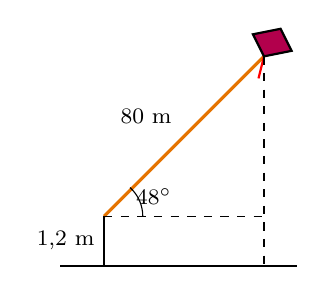
\begin{tikzpicture}[scale=0.7]
  % Mặt đất
  \draw[thick] (-0.5,0) -- (3.8,0);
  % Người thả diều
  \draw[thick] (0.3,0) -- (0.3,0.9);
  \node[left] at (0.3,0.45) {\footnotesize $1{,}2\text{ m}$};
  % Dây diều
  \draw[line width=1.1pt, orange!90!black] (0.3,0.9) -- (3.2,3.8);
  \node[above left] at (1.7,2.4) {\footnotesize $80\text{ m}$};
  % Con diều
  \draw[thick, fill=red!70!blue] (3.2,3.8) -- (3.0,4.2) -- (3.5,4.3) -- (3.7,3.9) -- cycle;
  \draw[thick, red] (3.2,3.8) -- (3.1,3.4); % Đuôi diều
  % Đường nằm ngang
  \draw[dashed] (0.3,0.9) -- (3.2,0.9);
  % Góc nghiêng 48 độ
  \draw (0.3,0.9) ++(0:0.7) arc (0:48:0.7);
  \node at (1.2,1.25) {\footnotesize $48^\circ$};
  % Đường gióng độ cao
  \draw[dashed] (3.2,3.8) -- (3.2,0);
\end{tikzpicture}
\end{minipage}

\vspace{1.5mm}
\textbf{Câu 18.} Một bồn hoa hình quạt tròn có bán kính $R = 12\text{ m}$ và góc ở tâm tương ứng là $45^\circ$. Tính diện tích của bồn hoa đó theo $\pi$ và làm tròn đến hàng phần mười (lấy $\pi \approx 3{,}14$, đơn vị: $\text{m}^2$).

\vspace{4mm}
\noindent
\textbf{\large II. TỰ LUẬN (3,0 điểm).} \textit{Thí sinh trình bày lời giải chi tiết vào tờ giấy thi.}

\vspace{2mm}
\textbf{Câu 19 (1,0 điểm).}
\begin{itemize}
  \item[a)] \textit{(0,5 điểm)} Giải hệ phương trình: $\begin{cases} 5x - 2y = 8 \\ 3x + 4y = 10 \end{cases}$.
  \item[b)] \textit{(0,5 điểm)} Cho biểu thức $M = \left( \dfrac{\sqrt{a}+1}{\sqrt{a}-1} - \dfrac{\sqrt{a}-1}{\sqrt{a}+1} \right) : \dfrac{4\sqrt{a}}{a-1}$ với $a > 0, a \ne 1$. Rút gọn biểu thức $M$.
\end{itemize}

\vspace{2mm}
\textbf{Câu 20 (1,5 điểm).} Cho tam giác nhọn $ABC$ nội tiếp đường tròn $(O; R)$ có các đường cao $BD, CE$ cắt nhau tại trực tâm $H$. Kẻ đường kính $AK$ của đường tròn $(O)$.
\begin{itemize}
  \item[a)] \textit{(0,75 điểm)} Chứng minh rằng bốn điểm $B, E, D, C$ cùng thuộc một đường tròn và tứ giác $BHCK$ là hình bình hành.
  \item[b)] \textit{(0,75 điểm)} Gọi $M$ là trung điểm của đoạn thẳng $BC$. Chứng minh rằng ba điểm $H, M, K$ thẳng hàng và $AH = 2 OM$.
\end{itemize}

\vspace{2mm}
\textbf{Câu 21 (0,5 điểm).}
\begin{itemize}
  \item[a)] \textit{(0,25 điểm)} Một công ty sản xuất lon nước ngọt hình trụ bằng nhôm có nắp đậy với thể tích $V = 54\pi\text{ cm}^3$. Gọi bán kính đáy lon là $r$ và chiều cao lon là $h$ (cm). Hãy tìm bán kính $r$ và chiều cao $h$ để diện tích toàn phần của lon nước ngọt là nhỏ nhất (nhằm tiết kiệm chi phí vỏ lon nhôm nhất)?
  \item[b)] \textit{(0,25 điểm)} Cho ba số thực dương $x, y, z$ thỏa mãn điều kiện $x + y + z = 3$. Tìm giá trị nhỏ nhất của biểu thức:
  \[
  S = \dfrac{x}{y^2 + 1} + \dfrac{y}{z^2 + 1} + \dfrac{z}{x^2 + 1}.
  \]
\end{itemize}

\vspace{4mm}
\begin{center}
\textbf{---------- HẾT ----------}\\
\textit{(Cán bộ coi thi không giải thích gì thêm)}
\end{center}

\end{document}
